


\section{Analysis}

\subsection{1. Impairments vs Rating analysis}

The analysis phase's goal was to evaluate the separability of star classes based on the features collected for each sample.
most of the work was exploratory and contained visualization of segments of the data in different forms to highlight change in distributions as function of change in feature/s

Figures  \ref{fig:mos_vs_stars} presents the distributions of different quality measures as a function of the Rate. The box plots in those figures shows that for lower rates the there are more samples with "bad" levels of quality measures than in high rates.
This insight suggest a relation between quality and rates that supplied the required justification to keep exploring in that direction.
In spite of the suggested direction by those figures , few notes most taken into account :
1. The charts hides out-liners ( lower 2.5\% , upper 2.5 \%) . because of the unbalanced distribution of rates, the out liners of the high Rates are mixed "overlay" the significance of the difference 
2. Most of the population of the Rates groups lays around the same values so the segregation suggested by the box plot distribution is only effective to extreme cases 

Sample of the distributions are presented below :

\paragraph{Rates vs. MOS}\label{rates-vs.-jitter}

As we can see, lower MOS values tend to appear in calls that were rated
as bad calls.

\begin{center}
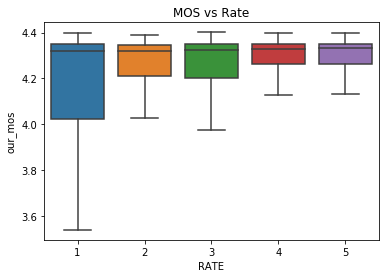
\includegraphics{figures/output_23_0.png}
\end{center}

\paragraph{Rates vs. jitter}\label{rates-vs.-jitter}

High jitter average values tend to appear in calls that were rated as
bad calls.

\begin{center}
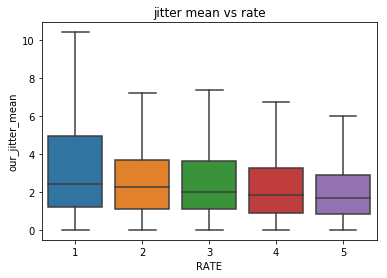
\includegraphics{figures/output_25_0.png}
\end{center}
    
\paragraph{Rates vs. RTT (latency)}\label{rates-vs.-rtt-latency}

High RTT average values tend to appear in calls that were rated as bad
calls.

 


\begin{center}
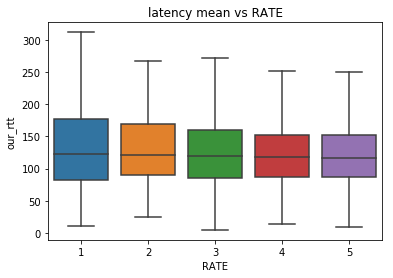
\includegraphics{figures/output_27_0.png}
\end{center}

    
\paragraph{Rates vs. Packet lost}\label{rates-vs.-packet-lost}

High packet lost percentage values tend to appear in calls that were
rated as bad calls.




\begin{center}
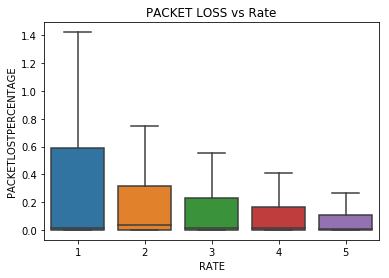
\includegraphics{figures/output_29_0.png}
\end{center}
    
\subsubsection{2. Call length}\label{call-length}

Another Promising dimension is the call length. we make an assumption that low quality calls will be over earlier than similar calls that have good quality. this assumption is supported by \ref{fig:Impairments_Length} visualizing the phenomena that shorter calls tend to have higher impairment values.

Combined with our basic thesis about the quality and Rates correlation requires that  we should see shorter calls in low rates.

\begin{figure}
    \centering
    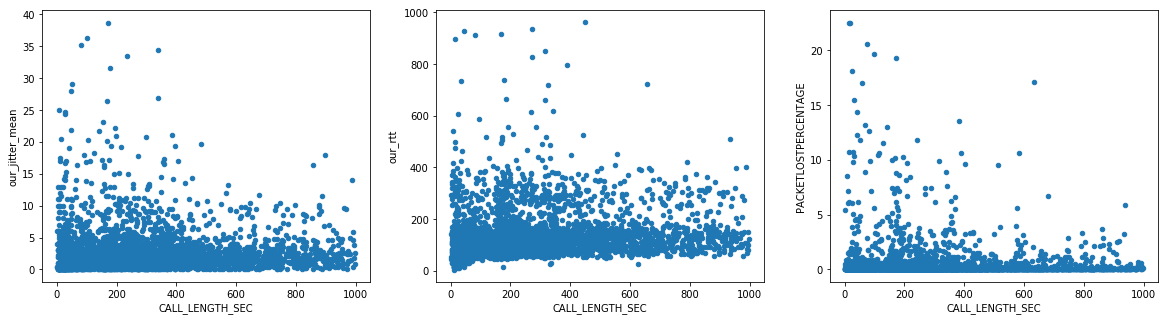
\includegraphics[scale=0.4]{figures/impairments_length.png}
    \caption{Impairments vs call length}
    \label{fig:Impairments_Length}
\end{figure}




Indeed, \ref{fig:Rates_call_length} shows that for shorter calls, the amount of '1' rated calls (bad) is high comparing to other rates whereas, in longer calls this amount declines   

\begin{figure}
    \centering
    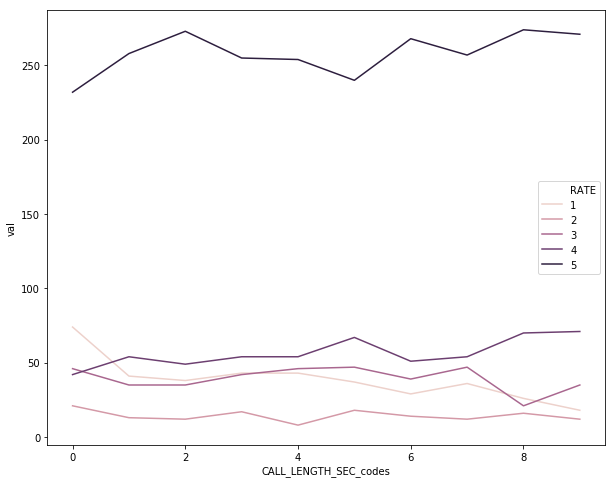
\includegraphics[scale=0.6]{figures/Rates_call_length_lines.png}
    \caption{Calls amount by rates vs Call length}
    \label{fig:Rates_call_length}
\end{figure}

\subsection{Analysis summery}
We have explored for a relation between calls data and their rates and found that statically there is some correlation ( level is not yet proven ) between different feature like call length and impairment on the Rate.
finally we present the full break down of impairments features we collected against the Rates in \ref{fig:all_arrays}

\begin{figure}
    \centering
    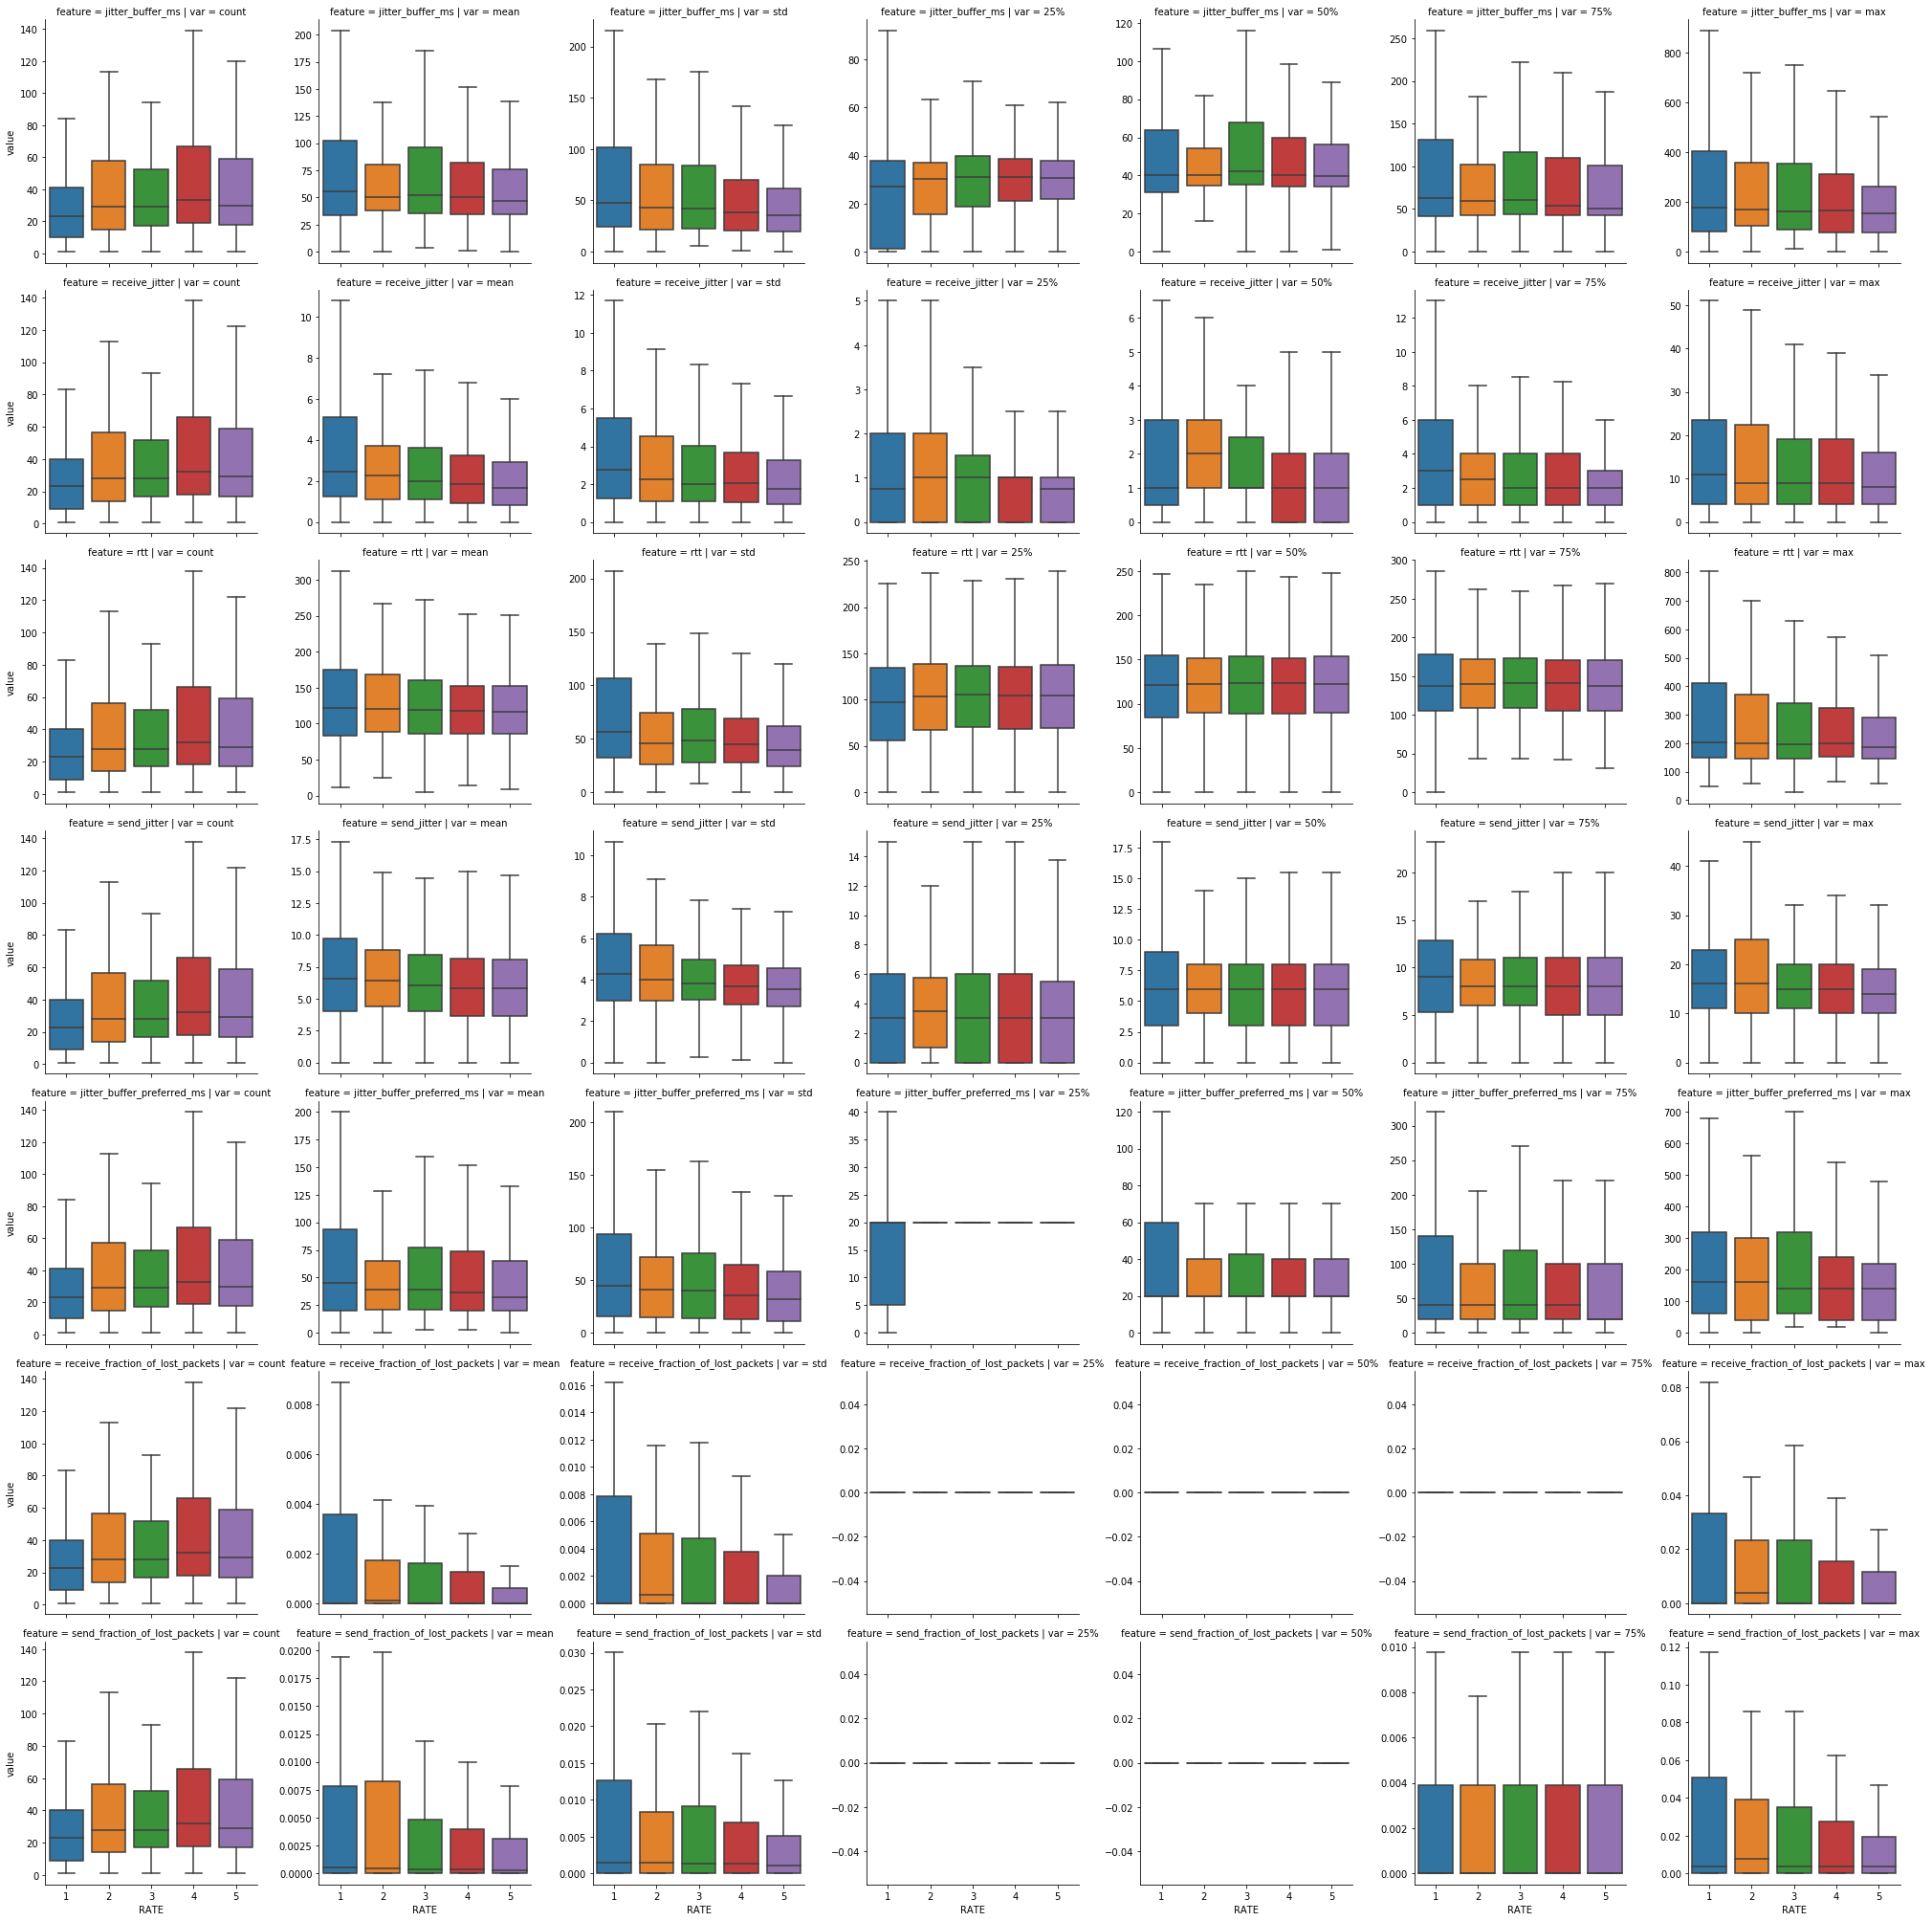
\includegraphics[scale=0.2]{figures/all_arrays.png}
    \caption{Impairments vs Rates}
    \label{fig:all_arrays}
\end{figure}
% %-------------------------Content------------------------
